\chapter{绪论} % 保持第一章标题

在全球战略格局深刻调整与新一轮科技革命加速演进的背景下,空天领域已成为关乎国家安全与发展的核心战略疆域\upcite{chen_hrrpgraphnet_2024, chen_radiallength_2024, pan_isar_2024, li_intell_2005, ju_anti_2016}。高超声速飞行器、大规模低轨卫星星座、隐身平台及无人机集群等新型空天目标的涌现,以其高动态、低探测、智能化等特征,对现有空天态势感知与防御体系构成严峻挑战\upcite{dong_high-speed_2025, rihaczek_theory_2000, zhang_bayesian_2020, he_anti_2024, sui_radar_2022}。雷达系统作为空天感知的核心手段,其获取的高分辨率距离像(High Resolution Range Profile, HRRP)、合成孔径雷达(Synthetic Aperture Radar,SAR)图像\upcite{luo_few-shot_2024, tai_few-shot_2022}与逆合成孔径雷达(Inverse-SAR,ISAR)图像\upcite{pan_isar_2024}是目标识别的关键特征\upcite{huang_noise-robust_2024, jian_survey_2022, zhang_patch-wise_2023, liu_radar_2011, xia_radar_2023-1}。近年来,深度学习显著提升了雷达自动目标识别(Radar Automatic Target Recognition, RATR)的性能,成为主流研究范式\upcite{ye_range-spread_2024, tai_few-shot_2022, gurbuz_data-driven_2018, dong_high-speed_2025, yang_radar_2024, liu_end--end_2022}。

然而,深度学习在RATR中的实际应用面临小样本问题的严峻瓶颈\upcite{luo_few-shot_2024, tai_few-shot_2022, liu_contrastive_2023}。实测雷达数据获取困难、目标类型与状态多样、数据标注成本高昂以及仿真与实测数据存在域差异等多重因素,导致高质量标注样本严重匮乏\upcite{xia_radar_2023}。这使得深度模型在小样本条件下极易过拟合,泛化能力不足\upcite{achille_task2vec_2019, rajeswaran_meta-learning_2019, tripuraneni_provable_2021}。同时,雷达一维像、二维像固有的对姿态角极端敏感\upcite{zhong_contrastive_2023, liu_scnet_2024}以及易受噪声、杂波影响导致低SNR\upcite{liu_end--end_2022, du_noise_2016, liu_prior-knowledge-guided_2024, pan_noise-robust_2013}等物理特性,进一步加剧了小样本学习的难度。为突破此困境,元学习,即“学会学习”的范式,因其能使模型从少量样本中快速学习和适应新任务而备受关注\upcite{li_meta-learning_2023, chen_evo-maml_2023, liu_few-shot_2021}。本研究聚焦小样本HRRP RATR,以元学习为核心框架,旨在探索应对噪声鲁棒性和角度敏感性挑战的创新方法,为提升领域技术水平做出一定贡献。

\section{研究背景与意义}
\label{sec:background_significance} % 添加标签以便引用
发展先进可靠的空天目标识别能力,对于维护国家安全、支撑军事行动和保障国家发展利益具有极其重要的战略意义\upcite{zhang_micro_2018, winters_target_2012, guo_method_2020, liu_radar_2025, liu_prior-knowledge-guided_2024}。目标识别是实现有效拦截、精确打击、威胁评估、意图判断等一系列后续军事和民事空天活动的基础环节\upcite{tai_few-shot_2022, Liu_ms_2021}。在现代战争呈现出的高动态、强对抗、复杂电磁环境以及无人化、智能化趋势下,快速、准确地判明目标的具体类型、型号、隶属乃至意图的能力,已成为夺取战场主动权、优化作战资源配置、提升体系作战效能的核心关键\upcite{li_intell_2005, ju_anti_2016, zhang_micro_2018}。俄乌冲突\upcite{ouyang_russia_2022, chen_american_2024}、巴以冲突\upcite{luo_is_2016}的经验反复印证,精确识别敌方高价值节点和主要威胁,对于战场态势实时生成、作战效果评估乃至冲突最终走向具有决定性影响。因此,先进的目标识别技术已成为现代军事体系不可或缺的关键使能技术。

\begin{figure}[h!]
    \centering
    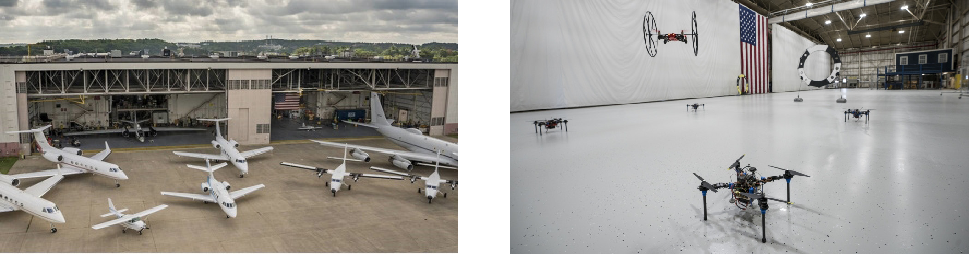
\includegraphics[width=\linewidth]{figures/kongzhong.pdf}
    \caption{现代战场非合作空天目标类型复杂多样、新类型不断涌现}
    \label{fig:hrrp_generation}
\end{figure}

鉴于空天目标识别的极端重要性,世界主要国家均将其置于国防科技发展的优先战略地位,投入巨大资源进行持续研发\upcite{williams_automatic_2000, rihaczek_theory_2000, roulston_radar_1997, rihaczek_man-made_1996}。西方国家在该领域起步较早,其发展历程展现出理论与工程紧密结合的特点,大致可分为数据库构建、模型探索与装备部署迭代三个阶段。在早期,以美国为代表的国家便着力于目标特征信号的雷达测量与数据库建设,例如利用夸贾林靶场的测量网将宽带雷达HRRP首次应用于目标识别\upcite{williams_automatic_2000, delaney_radar_2000},并建立了包括MSTAR在内的实测数据库及基于电磁仿真软件的大型仿真数据库\upcite{wu_american_2016};俄罗斯等国也同期开展了相关数据积累工作\upcite{yang_russia_2016, wang_russia_2022}。随后,在模型探索验证阶段,美国军事研发机构如DARPA、海军与空军实验室及顶尖高校如麻省理工学院、俄亥俄州立大学等\upcite{delaney_radar_2000, leminos_overview_2002}投入大量资源研究HRRP统计识别算法,为工程化应用奠定基础。进入21世纪,RATR技术已成为先进武器系统的必备能力\upcite{li_intell_2005},并广泛部署于各类平台,如英国的ASTOR、美国的E-8C“联合星”、P-3C以及“宙斯盾”等系统\upcite{wu_american_2016}。当前,各国研究的共同焦点仍是如何克服目标信号微弱、动态性强、背景扰动复杂、目标类型多样且不断演进以及敌方可能采取的智能化对抗措施等技术难题\upcite{wang_hyper_2022},并积极拥抱人工智能、大数据、多传感器协同等新兴技术,力求实现对空天目标的全时全域精确感知与深度认知。

\begin{figure}[h!]
    \centering
    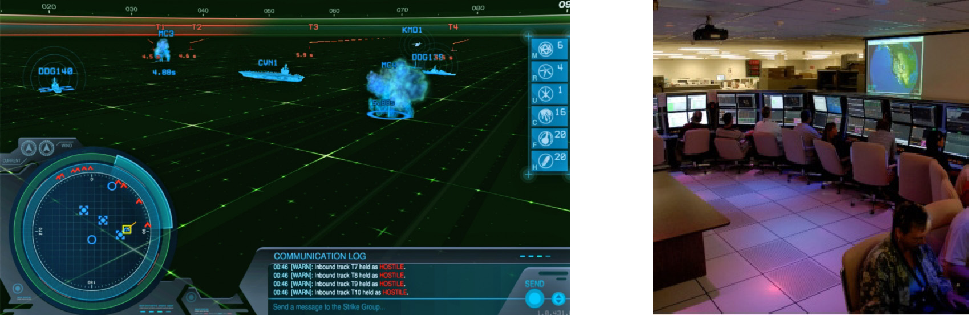
\includegraphics[width=\linewidth]{figures/military.pdf}
    \caption{美国麻省理工学院林肯实验室基于空天目标识别技术开展军事训练}
    \label{fig:hrrp_generation}
\end{figure}

对于我国而言,维护国家主权统一与领土完整、保障日益拓展的国家海外利益、有效应对来自空中、临近空间乃至外层空间的多维安全威胁、以及支撑海洋强国、航天强国等国家重大战略目标的顺利实现,均对我国的空天态势感知能力,特别是目标精确识别能力,提出了极为迫切且极高的现实要求\upcite{pan_zhuo_2006, tang_yi_2023}。我国面临的空天安全环境复杂,潜在威胁来源多样,涵盖从高性能隐身平台、战略武器,到临近空间与轨道空间的新型飞行器(如低轨卫星星座\upcite{gu_xinglian_2024})、各类卫星,再到“低小慢”无人机等不同维度\upcite{gong_21_2017, tian_zh_2016}。如果无法对这些潜在威胁进行及时、准确、可靠的识别,我国的国家空天预警与防御体系将存在关键短板,直接威胁国家安全。同时,随着我国国家利益的全球化和自身空天活动的日益频繁,保障海外利益安全和自身空天资产(例如应对空间碎片碰撞风险、非合作目标的异常接近或潜在攻击威胁\upcite{gu_xinglian_2024})稳定运行的需求也日益凸显。因此,大力发展自主可控、国际先进的空天目标自动识别技术体系,全面提升精确识别与深度理解能力,不仅是有效应对现实安全挑战的迫切需要,更是支撑国家重大战略实施、提升国家综合国力的基础性、战略性工程\upcite{huang_kongtian_2023}。

实现精确的空天目标探测识别依赖于多种传感技术手段的协同配合,包括光学、红外、以及雷达等。其中,雷达系统凭借其独特的主动探测能力、全天候全天时工作特性\upcite{tai_few-shot_2022, luo_few-shot_2024}、远距离探测优势\upcite{rihaczek_theory_2000}以及对目标物理结构和运动状态的独特敏感性,在空天感知体系中长期扮演着核心角色,尤其是在非合作目标探测与识别方面具有不可替代的作用\upcite{yang_radar-infrared_2024, guo_radar_2019, lagergren_deep_2020, rihaczek_man-made_1996, roulston_radar_1997}。雷达不仅能精确测量目标的运动学参数,更关键的是,通过对回波信号的幅度、相位、频率、极化等精细特征进行分析,能够反演目标的尺寸、形状、结构、材质等物理属性和姿态、微动等精细运动状态,为非合作目标的精确识别提供了不可或缺的信息来源\upcite{cui_template_2022, chen_radiallength_2024}。鉴于雷达在空天目标识别中的关键作用及其信号处理的独特性,本论文的研究工作聚焦于基于雷达信号的目标识别技术。

\begin{figure}[h!]
    \centering
    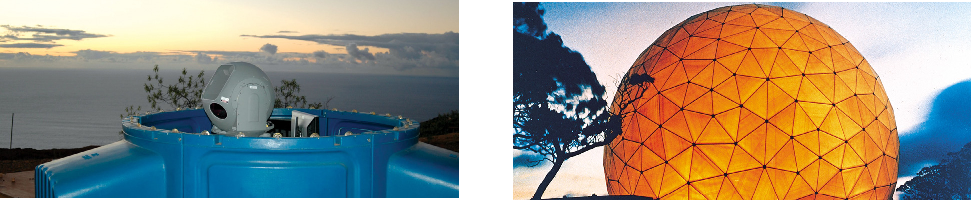
\includegraphics[width=\linewidth]{figures/reagan.pdf}
    \caption{马绍尔群岛美军罗纳德·里根弹道导弹防御试验场的红外、雷达检测跟踪识别系统}
    \label{fig:hrrp_generation}
\end{figure}

现代雷达技术的进步,特别是宽带信号处理和高分辨率成像技术的发展,极大地提升了雷达获取目标细节信息的能力\upcite{chen_hrrpgraphnet_2024, guo_method_2020}。宽带信号的应用提高了距离分辨率,能够分辨目标沿雷达视线(Line of Sight,LOS)的散射中心分布,形成HRRP\upcite{li_mtbc_2025, guo_radar_2025}。HRRP蕴含了目标一维结构信息,是RATR研究中最常用的一类特征\upcite{chen_radiallength_2024}。同时,SAR\upcite{luo_few-shot_2024, tai_few-shot_2022}与ISAR\upcite{pan_isar_2024}等成像技术能够生成目标的二维像,为识别提供了更丰富的信息。这些高分辨率技术的发展推动了RATR技术的演进。RATR技术大致经历了从早期的模板匹配\upcite{cui_template_2022},到中期的特征工程与浅层分类器(如基于子空间\upcite{shi_harmony_2010}、稀疏表示\upcite{liu_dictionary_2016}、流形学习\upcite{jiang_manifold_2016}、变换域特征\upcite{liu_few-shot_2021}的方法,以及基于优化或统计学习的分类器\upcite{du_radar_2011}),再到近十余年来由深度学习驱动的新阶段\upcite{ye_range-spread_2024, tai_few-shot_2022, gurbuz_data-driven_2018, dong_high-speed_2025, yang_radar_2024, liu_end--end_2022}。深度神经网络如卷积神经网络(Convoultional Nerual Network,CNN)\upcite{song_radar_2019}、循环神经网络(Recurrent Neural Network,RNN)\upcite{pan_radar_2022}及自编码器(Atuo-Encoder,AE)\upcite{wu_cae_2023}等凭借其强大的自动特征学习和非线性建模能力,实现了“端到端”的识别,在数据充足时显著超越了传统方法,成为当前研究的主流范式。国内研究也紧随这一趋势,并针对数据稀疏、模型扩展等工程问题进行了探索,例如使用生成对抗网络(Generative Adversarial Network, GAN)\upcite{zhou_gan_2022, song_limited_2024}合成数据和发展在线学习模型\upcite{huang_kongtian_2023}。

在众多的雷达目标特征中,HRRP作为一种一维表示,虽然信息量不如SAR、ISAR等雷达二维像丰富,但因其数据获取相对便捷、信号处理相对简单,且同样蕴含丰富的目标电磁物理特征,长期以来一直是该领域的基础研究对象和验证新算法的重要载体\upcite{chen_radiallength_2024}。因此,考虑到HRRP的基础性地位、其所面临问题的典型性以及研究课题范围的限制,本论文将主要围绕基于HRRP的目标识别展开,以期为解决更广泛的RATR问题提供基础性的方法探索和验证。

% --- 插入图1.1:HRRP角度敏感性示意图 ---
\begin{figure}[h!]
    \centering
    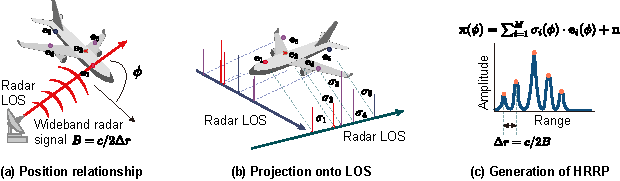
\includegraphics[width=\linewidth]{figures/hrrp_aspect.pdf}
    % \fbox{图 1.1: HRRP角度敏感性示意图 (占位符)}
    \caption{HRRP生成原理示意图}
    \label{fig:hrrp_generation}
\end{figure}

当前,将深度学习成功应用于实际复杂环境的RATR仍面临严峻的固有问题。第一个关键问题是真实电磁环境中的噪声与杂波影响\upcite{du_noise_2016, liu_prior-knowledge-guided_2024, pan_noise-robust_2013}。雷达信号不可避免地混杂背景杂波和系统噪声,这些影响严重降低信号信噪比(Signal-to-Noise Ratio, SNR),污染甚至淹没目标特征,对后续处理造成极大困难。如何在低信噪比条件下实现稳健识别,是衡量RATR系统实用价值的关键指标。第二个关键问题来源于雷达目标特征的内在复杂性与对观测条件的极端敏感性\upcite{zhong_contrastive_2023, liu_scnet_2024, liu_prior-knowledge-guided_2024}。电磁散射过程受多重因素耦合影响,导致HRRP这类一维像对目标姿态角变化极为敏感,即姿态敏感性(Aspect Sensitivity),微小变动即可引起特征剧烈畸变,严重影响识别稳定性\upcite{liu_prior-knowledge-guided_2024, li_prior_2024}(如图~\ref{fig:hrrp_generation}~和图~\ref{fig:hrrp_angle_sensitivity}~所示)。二维像同样存在角度依赖性,且成像质量受运动状态影响更加明显\upcite{zhang_isar_2021}。因此,从复杂、时变、敏感的雷达信号中提取稳定且具判别力的特征表示,始终是RATR领域的核心科学问题。第三个关键问题,也是当前最为突出的瓶颈,是高质量、大规模、标注完备的训练数据普遍严重匮乏,即小样本问题\upcite{luo_few-shot_2024, tai_few-shot_2022, liu_contrastive_2023, xia_radar_2023}。深度学习的性能高度依赖大数据训练,但在RATR领域,获取此类数据的成本高昂、实测获取难、目标类型动态变化、状态多样性导致样本需求巨大、数据标注困难且昂贵、仿真数据与实测数据间存在显著域差异等因素共同导致了训练样本的稀缺。这种数据稀缺性与深度模型的数据需求之间的矛盾,构成了当前RATR发展的核心困境\upcite{li_saratrx_2025}。在小样本条件下,深度模型极易过拟合,导致泛化能力严重不足。同时,现有方法在利用目标类别、功能、型号等语义信息方面尚显不足\upcite{chen_improving_2022, liu_remoteclip_2024}。在小样本或低分辨条件下,物理特征区分度不足时,融合语义信息有望提升识别精度和可靠性,但如何有效融合物理特征与语义信息仍是待探索的方向。第三个关键问题,也是当前最为突出的瓶颈,是高质量、大规模、标注完备的训练数据普遍严重匮乏,即小样本问题\upcite{luo_few-shot_2024, tai_few-shot_2022, liu_contrastive_2023, xia_radar_2023}。深度学习的性能高度依赖大数据训练,但在RATR领域,获取此类数据的成本高昂、实测获取难、目标类型动态变化、状态多样性导致样本需求巨大、数据标注困难且昂贵、仿真数据与实测数据间存在显著域差异等因素共同导致了训练样本的稀缺。这种数据稀缺性与深度模型的数据需求之间的矛盾,构成了当前RATR发展的核心困境\upcite{li_saratrx_2025}。在小样本条件下,深度模型极易过拟合,导致泛化能力严重不足。同时,现有方法在利用目标类别、功能、型号等语义信息方面尚显不足\upcite{chen_improving_2022, liu_remoteclip_2024}。在小样本或低分辨条件下,物理特征区分度不足时,融合语义信息有望提升识别精度和可靠性,但如何有效融合物理特征与语义信息仍是待探索的方向。

% --- 插入图1.1:HRRP角度敏感性示意图 ---
\begin{figure}[h]
    \centering
    \includegraphics[width=0.7\linewidth]{figures/aspect_tsne.pdf}
    % \fbox{图 1.1: HRRP角度敏感性示意图 (占位符)}
    \caption{HRRP样本角度敏感性的t-SNE可视化}
    \label{fig:hrrp_angle_sensitivity}
\end{figure}

% % --- 插入图1.2:噪声对HRRP的影响示意图 ---
% \begin{figure}[h!]
%     \centering
%     \fbox{图 1.2: 噪声对HRRP的影响示意图 (占位符)}
%     \caption{展示不同信噪比(SNR)条件下,噪声对HRRP样本形态的影响,说明低SNR下特征淹没和失真问题。}
%     \label{fig:hrrp_noise_effect}
% \end{figure}

面对上述固有问题与发展需求,RATR技术呈现出以下主要发展趋势:追求更高质量的特征信息获取\upcite{chen_hrrpgraphnet_2024};基于自监督\upcite{liu_attribute-informed_2025}、持续学习\upcite{liu_contrastive_2023}方法发展更智能、适应性更强的识别模型;基于物理知识引导的机器学习提升模型在复杂环境下的鲁棒性\upcite{liu_prior-knowledge-guided_2024, liu_scnet_2024};积极探索多源信息融合与协同识别\upcite{chen_improving_2022, liu_multi-polarization_2021};日益关注模型的可解释性、可信赖性与安全性\upcite{li_xai_2021};集中力量攻克小样本学习难题。其中针对小样本问题,元学习范式因其高效适应新任务的潜力而备受关注\upcite{liu_few-shot_2021},是本论文的核心思路。

综上所述,基于HRRP的RATR技术的发展机遇与问题并存。深度学习注入了新活力,但也使其在数据依赖如小样本问题、环境适应性如噪声、角度敏感性、特征复杂性等方面面临严峻制约。有效解决小样本学习问题,提升模型在真实复杂环境下的鲁棒性、泛化能力和快速适应能力,是当前RATR领域亟待突破的核心技术瓶颈。本研究正是紧密围绕此瓶颈,选择元学习作为主要的理论框架和技术途径,深入研究其在解决小样本雷达HRRP目标识别问题中的应用潜力,特别是在应对噪声影响、角度敏感性和语义信息利用等具体技术难点方面,提出针对性的创新方法,旨在为提升我国空天目标精确识别技术水平提供理论与技术储备。


\section{空天目标RATR技术研究现状}
\label{sec:related_work} % 添加标签
前文深入探讨了空天目标精确识别的战略紧迫性,并分析了雷达作为核心传感手段的优势、局限及发展趋势,特别指出了“小样本问题”是制约当前先进识别算法性能的关键瓶颈。在此基础上,本节将进一步聚焦于RATR领域如何应对数据稀缺性的挑战。我们将首先回顾传统RATR方法为何在处理复杂性和小样本问题上存在固有的局限性;接着,阐述深度学习方法如何作为一种更强大的范式被引入RATR领域,并分析其在带来性能提升的同时,如何使得小样本问题变得更为突出和关键;最后,在此背景下,系统梳理当前专门针对小样本RATR的研究现状、主要技术途径及其面临的核心挑战。

在深度学习技术广泛应用之前,RATR研究自上世纪50年代起步\upcite{williams_automatic_2000, delaney_radar_2000, leminos_overview_2002},至90年代中期已形成包括数据预处理、特征提取和分类器设计的基本框架\upcite{li_using_1993, mitchell_overview_1994, zyweck_radar_1996},其发展主要沿着两条技术路径:基于模板匹配\upcite{cui_template_2022}和基于特征工程与浅层或统计分类器\upcite{jian_survey_2022, liu_radar_2008, du_radar_2011}。模板匹配方法通过将待测目标特征与预建模板库进行比对来识别,原理直观。然而,HRRP数据固有的姿态、平移和幅度敏感性,加之目标多样性与模板库难以完备的现实,使得该方法在面对姿态剧变或样本稀少、无法构建代表性模板库的小样本条件下,其性能和鲁棒性显著不足\upcite{cui_template_2022, jian_survey_2022}。

为了克服这些限制,研究重心转向了特征工程路线。该路线旨在通过人工设计对姿态、噪声等特定变化相对不敏感的稳健特征,再结合各类分类器进行判决\upcite{jian_survey_2022}。这一方向衍生出多种具体方法,如通过线性判别分析(Linear Discriminant Analysis ,LDA)\upcite{liu_radar_2008}、主成分分析(Principal Component Analysis,PCA)\upcite{zhang_isar_2021}流形学习进行降维;利用字典学习提取稀疏表示特征\upcite{guo_method_2020, wu_cae_2023};挖掘HRRP序列的时空连续性信息如隐马尔可夫模型(Hidden Markov Model,HMM)\upcite{du_radar_2011, tu_novel_2019}、多模态模型\upcite{pan_noise-robust_2013}、受限玻尔兹曼机(Restricted Boltzmann Machine,RBM)\upcite{liu_experimental_2020};采用核方法处理非线性问题\upcite{zhang_micro_2018};以及基于统计模型如高斯混合模型(Gaussian Mixed Model,GMM)\upcite{pan_noise-robust_2013}、自适应高斯分类器\upcite{pan_noise-robust_2013}进行贝叶斯决策\upcite{jian_survey_2022}。

尽管特征工程通过信息抽象提升了一定的灵活性和鲁棒性,但其成功严重依赖于特征设计的质量。这不仅需要深厚的领域知识、耗时费力,而且设计出的特征往往泛化能力有限\upcite{jian_survey_2022}。HRRP的多种敏感性进一步加剧了设计通用稳健特征的难度。特别是在小样本条件下,缺乏足够数据指导特征设计与验证,难以获得真正具有普适判别力的特征\upcite{jian_survey_2022, wen_hrrp_2020}。同时,无论是浅层的支持向量机(Support Vector Machine,SVM)、K近邻(K Nearest Neighbours,KNN)方法还是统计模型,传统分类器有限的模型容量也难以充分捕捉雷达数据内在的高度非线性复杂关系,限制了识别性能的上限\upcite{jian_survey_2022}。因此,传统方法在特征表示能力、模型泛化性、自动化程度以及应对小样本挑战的能力上均存在明显瓶颈\upcite{jian_survey_2022, liu_radar_2011},难以满足现代空天目标识别任务对高精度、高鲁棒性、高适应性的迫切需求\upcite{li_intell_2005, huang_kongtian_2023}。

% % --- 插入图1.3:传统RATR vs 深度学习RATR ---
% \begin{figure}[h!]
%     \centering
%     \fbox{图 1.3: 传统RATR与深度学习RATR流程对比 (占位符)}
%     \caption{对比展示传统RATR(人工特征提取 + 浅层分类器)与深度学习RATR(端到端学习)的基本流程示意图。}
%     \label{fig:ratr_comparison}
% \end{figure}

近十年来,深度学习凭借其从大规模数据中自动学习层次化特征表示的卓越能力,在计算机视觉等领域取得革命性成功后,也被迅速引入RATR领域\upcite{liu_experimental_2020, wu_high-resolution_2019, liu_radar_2025}。以CNN\upcite{song_radar_2019}、RNN\upcite{pan_radar_2022}及其变种\upcite{yang_radar_2024, zeng_radar_2022}、AE\upcite{wu_cae_2023}、长短时记忆网络(Long-Short Term Memory,LSTM)\upcite{tu_novel_2019, jithesh_lstm_2017}、图神经网络(Graph Neural Network,GNN)\upcite{chen_hrrpgraphnet_2024}以及近年备受关注的Transformer架构\upcite{vaswani_attention_2017, gao_polarimetric_2024}为代表的深度模型,能直接处理雷达一、二维像数据实现“端到端”识别流程,在数据相对充分的条件下,展现出超越传统方法的性能潜力\upcite{liu_attribute-informed_2025},标志着RATR技术进入了崭新的发展阶段。

然而,深度学习的强大性能与其大规模标注数据驱动的特性是一体两面\upcite{thanapol_reducing_2020}。虽然RATR领域的数据稀缺问题由来已久,但在深度学习范式下,这个问题变得尤为尖锐和关键。深度模型通常包含数百万甚至更多的参数,需要海量的、多样性的标注样本进行有效训练才能避免过拟合,学习到具有良好泛化能力的特征表示\upcite{liu_attribute-informed_2025}。但在RATR领域,如前文所述,获取大规模、高质量、标注完备的实测数据面临着成本、限制、目标多样性、状态多变性、标注难度以及仿真数据域差异等多重现实障碍\upcite{li_saratrx_2025}。这种深度模型对数据的强依赖性与雷达数据获取的固有困难之间的矛盾,使得小样本问题从一个普遍存在的挑战,升级为制约深度学习RATR技术实用化、发挥其全部潜力的核心瓶颈。现有深度学习模型应用于小样本RATR场景,往往导致模型训练不足、过拟合严重,识别性能远达不到预期。因此,如何在深度学习框架下有效应对数据稀缺性,成为RATR领域亟待解决的关键科学问题,直接催生了针对性的小样本学习(Few-shot Learning,FSL)研究方向\upcite{li_libfewshot_2023, luo_closeragain_2023}。

\section{小样本RATR技术研究现状与关键问题} % 修改标题
\label{sec:fsl_challenges} % 添加标签
面对传统方法的局限以及深度学习范式下凸显的小样本瓶颈,FSL已成为推动RATR技术发展的关键研究方向\upcite{liu_few-shot_2021, li_libfewshot_2023, Liu_ms_2021}。FSL旨在使模型具备从极少量标注样本中学习并泛化到新类别或新任务的能力\upcite{luo_closeragain_2023, vinyals_matching_2016}。近年来,研究者们已将多种源于通用机器学习领域的FSL策略引入小样本RATR研究,并针对雷达数据的特性进行了初步的适应与发展\upcite{kong_few-shot_2023, tai_few-shot_2022, luo_few-shot_2024}。本小节将首先概述FSL在RATR领域应用的主流技术途径,然后重点剖析本研究所关注的三个关键问题及其现有研究的不足之处。

% --- 插入图1.5:雷达小样本RATR技术研究现状 ---
\begin{figure}[h]
    \centering
    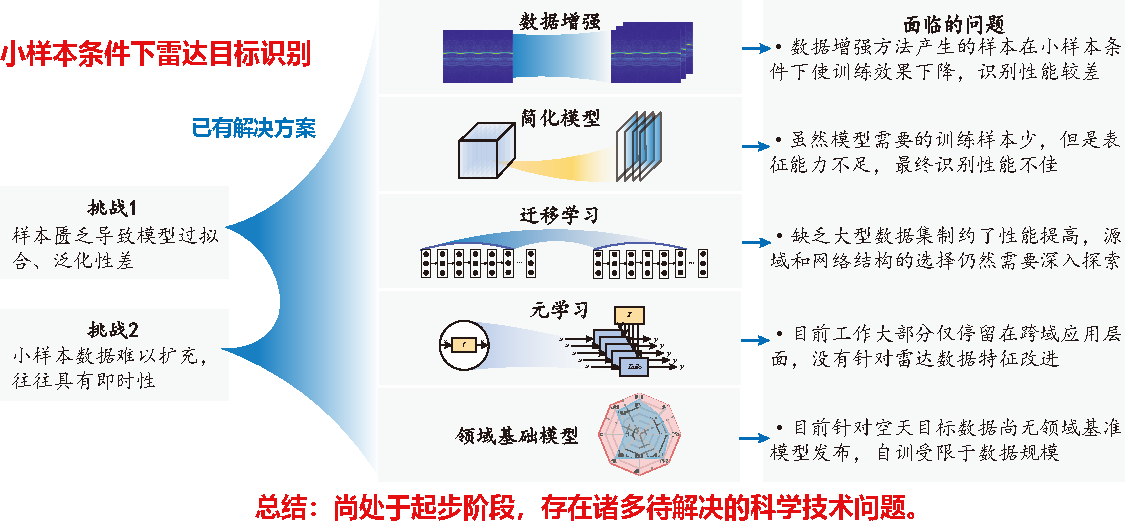
\includegraphics[width=\linewidth]{figures/review.pdf} % 假设图文件存在
    % \fbox{图 1.5: 雷达小样本RATR技术研究现状 (占位符)}
    \caption{雷达小样本RATR技术研究现状}
    \label{fig:meta_learning_paradigms}
\end{figure}

当前应用于小样本RATR的主流FSL技术途径大致可分为以下几类:

(1)数据增广

作为应对数据稀疏问题的常用手段,数据增广(Data Augmentation,DA)旨在通过对现有样本进行变换或利用生成模型合成新样本来扩充训练集,以期提升模型的泛化能力\upcite{xu_effective_2024, song_limited_2024}。在RATR领域,除了应用传统的几何变换、添加模拟噪声等简单操作外,基于深度生成模型,特别是GAN进行雷达样本合成以实现数据扩充的技术受到了广泛关注\upcite{zhou_gan_2022, song_limited_2024}。针对HRRP样本生成,Huang等\upcite{huang_recognition_2021}提出了一种识别感知的生成框架,通过分解与重组信号特征来生成具有判别力的HRRP样本,以提高识别系统性能。在SAR图像生成方面,Zeng等\upcite{zeng_gan_2024}提出了角度变换GAN(ATGAN),将生成任务重构为图像到图像的转换问题,实现了方位角可控且细节保持良好的SAR目标图像生成。针对ISAR图像数据的不完整性,Zhang等\upcite{zhang_gan_2024}设计了一种由粗到精的两阶段插值网络C2FIPNet,结合流估计与GAN,用于生成具有中间方位角的ISAR图像,以增强数据集并提升识别精度。然而,数据增广策略亦存在固有局限性。其一是简单的变换方法难以充分模拟雷达数据在真实场景下可能经历的复杂变化,例如由目标微动、散射中心迁移等引起的非线性效应\upcite{jian_survey_2022, guo_influence_2013}。其二,基于深度生成模型的方法虽然潜力巨大,但生成样本的保真度、多样性及与真实数据分布的一致性仍是挑战,训练过程中可能面临模式坍塌、难以控制生成样本属性等问题\upcite{xu_effective_2024, song_limited_2024}。更为关键的是,无论是变换已有样本还是生成新样本,现有数据增广主要依赖于已观测到的数据信息,并未引入关于未知类别目标的本质知识,因此其在提升模型对全新、未见类别的泛化识别能力方面作用有限\upcite{Liu_ms_2021}。
一是基于数据增广的策略\upcite{xu_effective_2024, song_limited_2024}。作为应对数据稀疏问题的常用手段,数据增广旨在通过对现有样本进行变换或利用生成模型合成新样本来扩充训练集,以期提升模型的泛化能力。在RATR领域,除了应用传统的几何变换、添加模拟噪声等简单操作外,基于深度生成模型,特别是GAN进行雷达样本合成以实现数据扩充的技术受到了广泛关注\upcite{zhou_gan_2022, song_limited_2024}。针对HRRP样本生成,Huang等\upcite{huang_recognition_2021}提出了一种识别感知的生成框架,通过分解与重组信号特征来生成具有判别力的HRRP样本,以提高识别系统性能。在SAR图像生成方面,Zeng等\upcite{zeng_gan_2024}提出了角度变换GAN(ATGAN),将生成任务重构为图像到图像的转换问题,实现了方位角可控且细节保持良好的SAR目标图像生成。针对ISAR图像数据的不完整性,Zhang等\upcite{zhang_gan_2024}设计了一种由粗到精的两阶段插值网络C2FIPNet,结合流估计与GAN,用于生成具有中间方位角的ISAR图像,以增强数据集并提升识别精度。然而,数据增广策略亦存在固有局限性。其一是简单的变换方法难以充分模拟雷达数据在真实场景下可能经历的复杂变化,例如由目标微动、散射中心迁移等引起的非线性效应\upcite{jian_survey_2022, guo_influence_2013}。其二,基于深度生成模型的方法虽然潜力巨大,但生成样本的保真度、多样性及与真实数据分布的一致性仍是挑战,训练过程中可能面临模式坍塌、难以控制生成样本属性等问题\upcite{xu_effective_2024, song_limited_2024}。更为关键的是,无论是变换已有样本还是生成新样本,现有数据增广主要依赖于已观测到的数据信息,并未引入关于未知类别目标的本质知识,因此其在提升模型对全新、未见类别的泛化识别能力方面作用有限\upcite{Liu_ms_2021}。

(2)迁移学习

迁移学习(Transfer Learning,TL)的核心思想是将从数据充足的源域(如仿真数据、光学图像或大规模通用数据集)学习到的知识迁移应用于数据稀缺的目标域(如实测雷达数据)\upcite{wen_hrrp_2020, tai_few-shot_2022}。在RATR中,常见的做法是利用源域数据预训练深度模型,然后在目标域的少量样本上进行微调\upcite{wen_hrrp_2020, li_mtbc_2025}。Wen等\upcite{wen_hrrp_2020}利用具有完整方位角信息的辅助HRRP数据来提升模型在方位角缺失情况下的识别性能;Tan等\upcite{tai_few-shot_2022}则探索了从光学图像域向SAR图像域的知识迁移。然而,迁移学习的有效性高度依赖于源域与目标域之间的相关性及相似性\upcite{wen_hrrp_2020}。雷达应用中普遍存在显著的域偏移问题,这源于传感器差异、成像条件变化、目标姿态敏感性、噪声特性不同以及仿真数据与实测数据间的鸿沟等\upcite{wen_hrrp_2020, liu_attribute-informed_2025},这些因素都会严重限制知识迁移的效果,导致模型在目标域性能下降\upcite{wen_hrrp_2020}。
% 为缓解域偏移问题,领域自适应(Domain Adaptation, DA)技术致力于显式地减小源域和目标域之间的分布差异,以提升模型的跨域泛化能力\upcite{li_mtbc_2025, li_episodic_2019}。这通常通过两种主要途径实现:一是在特征空间中对齐不同域的数据分布,例如通过最小化最大均值差异(Maximum Mean Discrepancy, MMD)或进行相关性对齐;二是利用对抗学习机制,训练一个域判别器来区分样本来源,同时优化特征提取器以生成令域判别器混淆(即域不变)的特征\upcite{zhong_contrastive_2023, xu_effective_2024}。例如,文献\upcite{li_episodic_2019}提出了一种情景训练(Episodic Training)方法,它在训练过程中模拟域之间的转换,从而增强模型对于未见域的泛化性能;文献\upcite{zhong_contrastive_2023}针对HRRP方位角缺失问题(可视为一种域偏移),运用对比自监督学习框架来提取对目标方位角变化具有不变性的特征表示;而文献\upcite{xu_effective_2024}则采用了对比对抗训练(CAT)策略来生成更具挑战性的HRRP增广样本,通过提升模型对困难样本的辨识能力间接增强了其在不同数据分布下的鲁棒性。

(3)元学习

元学习(Meta-Learning),常被称为“学会学习”(learning to learn),其核心目标是使模型能从一系列相关的训练任务中习得跨任务的通用知识或学习策略,进而能够在面对仅有少量标注样本的新任务时,快速适应并实现有效泛化\upcite{finn_model-agnostic_2017, li_libfewshot_2023, liu_few-shot_2021}。这一思想可以追溯到对归纳偏置学习的研究\upcite{baxter_model_2000},并在深度学习时代得到了蓬勃发展。元学习通常采用“任务式”(Task-based)的训练框架,又叫S/Q Training或Episodic Training\upcite{li_episodic_2019, vinyals_matching_2016},模拟小样本学习的场景。

% --- 插入图1.4:Few-Shot Learning 任务示意图 ---
\begin{figure}[h!]
    \centering
    % \fbox{图 1.4: Few-Shot Learning 任务设置示意图 (占位符)}
    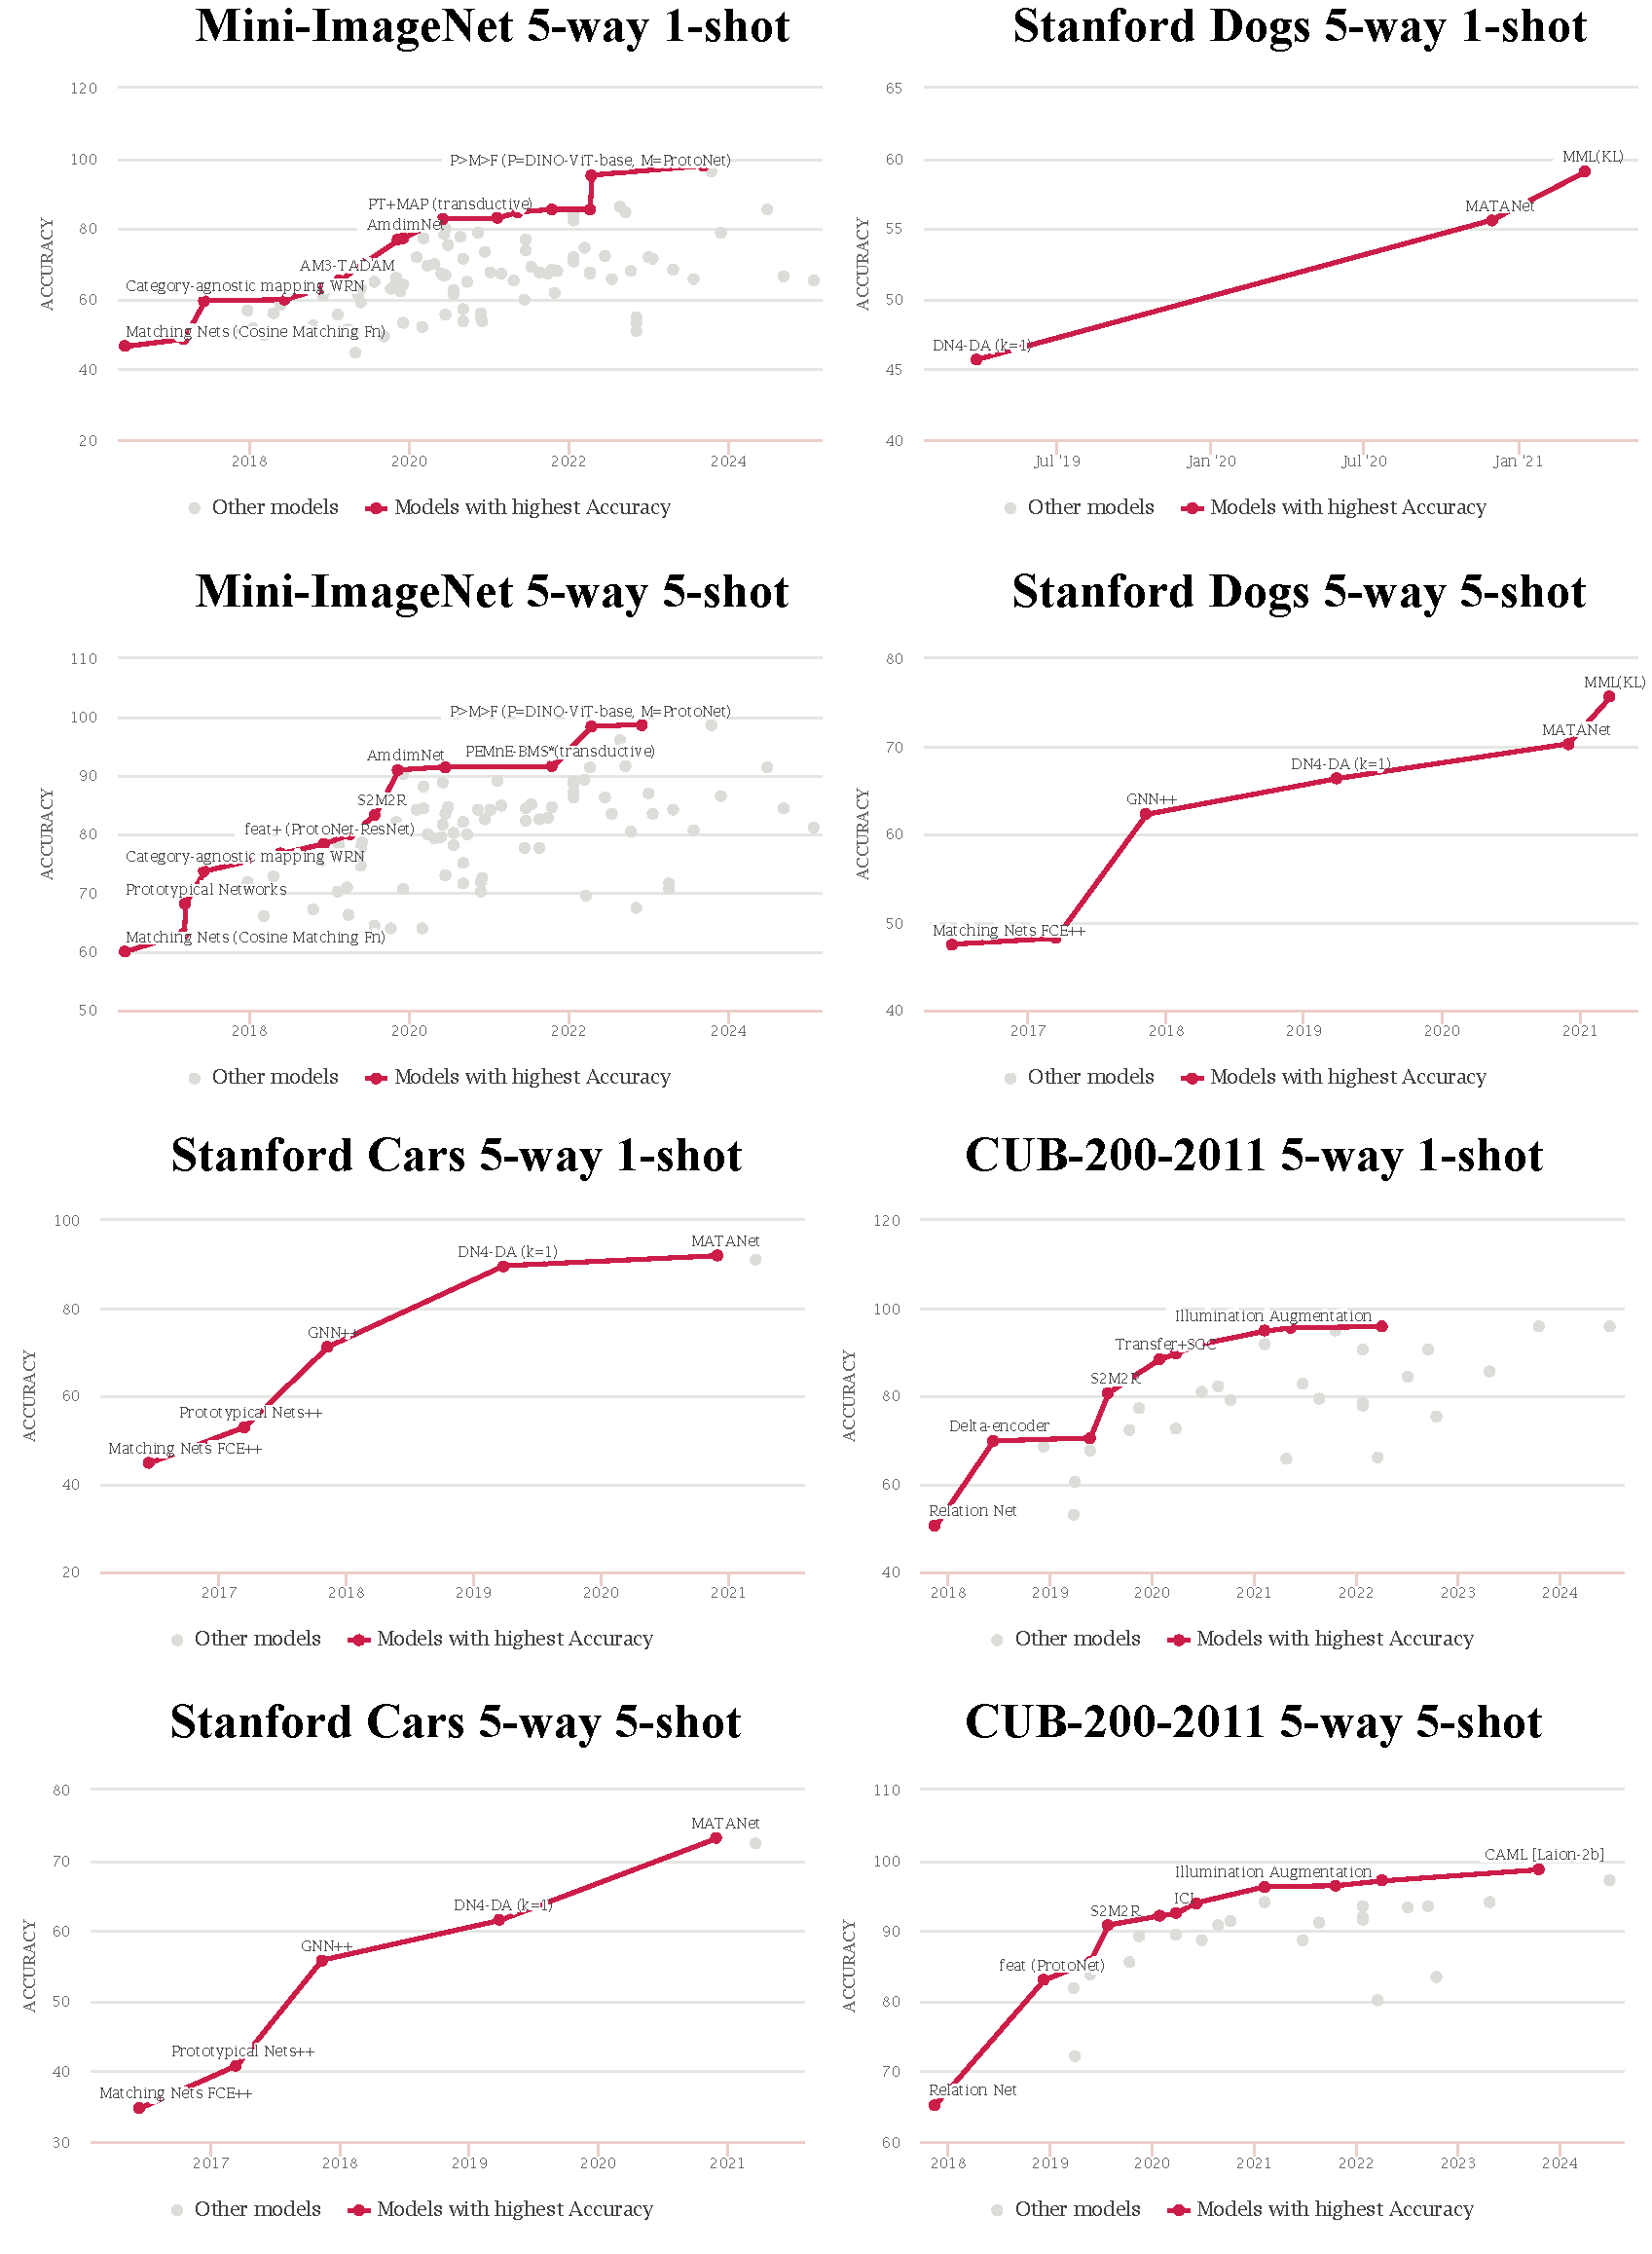
\includegraphics[width=0.9\linewidth]{figures/fsl.pdf}
    \caption{小样本学习在光学领域进展迅速}
    \label{fig:fsl_task}
\end{figure}

在当前的元学习范式下,主要形成了两大类主流方法:一类是基于优化的元学习。其代表性工作是Finn等\upcite{finn_model-agnostic_2017}提出的模型无关元学习(Model-Agnostic Meta-Learning, MAML),它旨在寻找一个对任务损失极其敏感的初始化参数,使得模型在新任务上只需通过少量梯度更新步骤就能快速达到良好的性能\upcite{raghu_rapid_2020, zhou_task_2021}。后续研究也围绕MAML的计算效率和稳定性进行了改进,例如OpenAI\upcite{nichol_reptile_2018}提出的Reptile、Yang\upcite{yang_few-shot_2022}等提出的一阶近似方法以及Rajeswaran等\upcite{rajeswaran_meta-learning_2019}提出的隐式梯度等。另一类是基于度量的元学习。这类方法的核心不在于优化模型参数本身,而是学习一个优质的嵌入空间以及一个有效的相似性度量函数\upcite{vinyals_matching_2016, snell_prototypical_2017}。目标是在这个空间中,能够基于少量支持样本有效地对查询样本进行分类。早期的代表性工作如Vinyals等\upcite{vinyals_matching_2016}提出的匹配网络(Matching Networks, MN)利用注意力机制来计算查询样本与支持样本的相似度。随后,Snell等\upcite{snell_prototypical_2017}的原型网络(Prototypical Networks, ProtoNet)提出了一种更简洁的思路,即计算每个类别的原型(通常是支持集样本嵌入的均值),然后基于查询样本嵌入与各类别原型的距离进行分类,因其简单有效而被广泛应用于包括RATR在内的诸多领域\upcite{tian_open_2022, liu_contrastive_2023, li_few-shot_2023}。此外,Sung等\upcite{sung_relation_2018}提出的关系网络(Relation Network,RelationNet)则通过学习一个神经网络来直接建模样本对之间的关系得分。总体而言,元学习为系统性地解决小样本问题提供了一个强大的理论框架,其“快速适应”和“从少量样本中学习”的核心理念与RATR在非合作目标、数据获取困难等实际场景下的迫切需求高度契合\upcite{liu_multi-polarization_2021},近年来已成为小样本RATR研究的重要方向,展现出巨大的应用潜力\upcite{liu_few-shot_2021, kong_few-shot_2023, li_prior_2024}。

随着元学习在光学图像小样本识别领域取得显著成功,一部分研究者开始将其引入小样本RATR问题中。这些初步尝试探索了不同元学习策略的应用:例如,高飞等\upcite{gao_metric_2021}提出基于度量学习的SAR识别方法;Wang等\upcite{wang_meta_2021}结合概率推断与元学习进行仿真到实测的知识迁移;Fu等\upcite{fu_meta_2022}则将Meta-SGD与迁移学习结合。然而,当前基于元学习的RATR工作多数仍停留在直接应用层面,即将在光学图像识别中验证有效的元学习算法直接应用于雷达数据,往往未能充分考虑雷达信号固有的物理特性和独特的敏感性\upcite{jian_survey_2022, guo_influence_2013, Liu_ms_2021}。这种“直接移植”忽略了雷达数据的领域特殊性,导致算法性能常常无法达到预期\upcite{Liu_ms_2021}。因此,本文认为,必须深入结合雷达数据的特有属性对现有元学习框架进行针对性的改进与设计,才能发展出真正适合小样本RATR任务的算法,从而有效利用元学习的快速学习能力和强表征能力,提升识别准确率和泛化性能。由于课题研究的时间限制以及HRRP在RATR中的基础性和广泛应用,本文工作聚焦在基于HRRP的RATR研究上。具体而言,将这些通用的元学习方法应用于复杂的HRRP RATR场景时,仍面临一系列严峻的、与雷达数据特性相关的具体问题,这正是本文需着力解决的关键:

\textbf{其一是低信噪比与复杂噪声环境下的鲁棒识别问题。}
雷达信号极易受到各种噪声、杂波的影响,导致SNR显著降低\upcite{liu_end--end_2022, du_noise_2016, liu_prior-knowledge-guided_2024, pan_noise-robust_2013}。在小样本条件下,噪声的存在不仅进一步模糊了目标本身微弱的结构信息,加剧了从有限数据中提取稳定判别特征的难度,更容易导致模型在噪声上过拟合,从而使得识别性能急剧恶化\upcite{jian_survey_2022}。传统的抗噪声方法,如Du等\upcite{du_noise_2016}基于散射点匹配的算法,Pan等\upcite{pan_noise-robust_2013}统计模型修正,以及通用深度学习中旨在提升鲁棒性的设计(例如引入残差连接\upcite{guo_radar_2019, huang_noise-robust_2024}、注意力机制\upcite{chen_target-attentional_2022}或采用去噪自编码器\upcite{guo_method_2020, wu_cae_2023}),往往依赖于对噪声模型的先验假设或需要充足的数据来学习噪声的统计特性。然而,雷达系统在真实作战环境中面临的噪声往往是复杂、非平稳、未知且随场景动态变化的。现有的通用元学习方法的标准框架大多缺乏针对雷达领域常见的复杂噪声环境进行鲁棒性设计。具体而言,标准的元学习任务构建过程通常不涉及跨任务的噪声水平或类型变化模拟,其泛化性可能对测试时遇到的未知噪声不鲁棒;度量学习所构建的嵌入空间也可能因噪声干扰而变得不再可靠,使得映射规则失效。因此,如何在样本极其有限的情况下,使元学习模型具备对未知或变化的复杂噪声的自适应鲁棒识别能力,是将其成功应用于实际RATR场景的一个亟待解决的关键难题。

\textbf{其二是雷达特征的角度敏感性导致模型泛化困难的问题。}
姿态角的微小变化就可导致HRRP样本的形态结构发生剧烈且高度非线性的变化,使得同一目标在不同角度下的样本间差异有时甚至会超过不同类别目标之间的差异\upcite{zhong_contrastive_2023, wen_hrrp_2020, dong_high-speed_2025}。这种现象严重违反了机器学习分类任务中“类内紧凑、类间分离”的基本假设,构成了基于HRRP进行目标识别的固有核心物理瓶颈\upcite{jian_survey_2022}。传统方法,如试图设计角度不敏感特征或构建精细的多姿态模板库\upcite{cui_template_2022},在小样本或宽角度范围下效果有限且代价高昂。深度学习方法,例如利用RNN、LSTM处理HRRP序列\upcite{pan_radar_2022, jithesh_lstm_2017, tu_novel_2019}或设计特定的CNN结构\upcite{song_radar_2019},虽然在数据充足时能学习到一定的角度依赖关系,但在小样本条件下,它们难以从稀疏、可能分布不均的角度样本中充分捕捉复杂的非线性角度变化规律,导致跨角度泛化能力显著下降\upcite{wen_hrrp_2020, liu_scnet_2024}。现有的通用元学习方法,其有效性通常也建立在每个小样本任务内部的样本具有一定程度相似性的假设之上。HRRP的强角度敏感性恰恰打破了这一假设,给元学习带来了巨大挑战:对基于优化的方法,学习一个既能快速适应新类别、又能对剧烈角度变化保持稳健的初始化参数变得异常困难;对基于度量的方法,学习一个能将同一目标不同角度的样本有效聚类、同时区分开不同目标的嵌入空间也极具挑战性。虽然已有少量工作如Wen等\upcite{wen_hrrp_2020}和Zhong等\upcite{zhong_contrastive_2023}尝试将FSL思想应用于HRRP的角度缺失或变化问题,Liu等\upcite{liu_prior-knowledge-guided_2024, liu_scnet_2024}也探索了结合物理先验知识提升模型角度鲁棒性的方法,但如何在元学习框架下,系统性地、有效地克服HRRP的强角度敏感性,特别是在角度跨度大、样本极其稀疏的情况下,实现对宽角度范围或未知角度目标的可靠识别,仍然是小样本RATR领域亟待攻克的另一个核心技术难题。

\begin{figure}[h!]
    \centering
    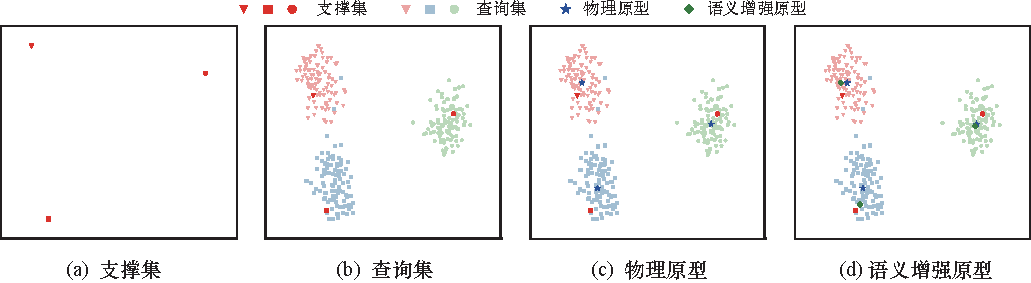
\includegraphics[width=\linewidth]{figures/yuyi.pdf}
    \caption{MiniImageNet 数据集上语义嵌入方法SemFew原型增强效果的t-SNE可视化\upcite{zhang_simple_2024}}
    \label{fig:yuyi}
\end{figure}

\textbf{最后是在特征判别性不足场景中难以利用语义信息,导致混淆的问题。}
当每类训练样本极少时,单纯依赖从雷达物理信号学习到的底层特征表示,可能不足以有效区分结构相似、散射特性接近的不同目标类别。Liu等\upcite{liu_multi-polarization_2021}基于多极化HRRP数据融合实现了小样本条件下HRRP的有效识别,但是未从电磁散射特性相近的本质解决问题,导致特征判别性不足的问题在高相似度目标混杂场景中可能更加突出。目标的语义信息,即关于目标的高层抽象知识,能提供独立于物理特征的重要补充判别线索\upcite{chen_improving_2022}。在通用计算机视觉领域,将语义信息融入FSL如通过语义嵌入指导度量学习\upcite{zhu_kan_2021, xu_2022_cvpr, zhang_simple_2024}或利用语义信息生成分类器权重\upcite{dos_cross_2023}已在零样本学习(Zero-Shot Learning, ZSL)和少样本学习中取得显著效果。然而,在RATR领域,系统性研究如何获取、表示雷达目标特有的语义信息(例如,基于目标的物理结构、功能用途、甚至作战意图等),并将其有效融入小样本框架的研究尚处初级阶段\upcite{liu_attribute-informed_2025}。Chen等\upcite{chen_improving_2022}提出基于BERT、GloVe等自然语言处理模型对遥感场景的标签信息进行语义嵌入,但这种基于通用语言模型的语义特征可能缺乏雷达目标识别任务所需的领域知识特异性。探索如何利用预训练的、具备强大跨模态理解能力的基础模型(Foundation Model)\upcite{li_saratrx_2025, liu_remoteclip_2024},并结合目标的结构、功能等语义信息来增强小样本雷达识别的判别能力,成为一个值得关注且具有潜力的新方向。

综上所述,尽管FSL为RATR带来了新思路,但现有通用方法在面对噪声影响、角度敏感性以及特征判别性不足这三大关键问题时仍存局限。针对这些特定问题设计定制化的、能利用雷达数据特性和物理先验的小样本学习(特别是元学习)方法,是推动该领域发展的关键。本论文正是基于此认识,聚焦于利用元学习框架,分别针对性地提出创新解决方案。

\section{本文主要研究内容与结构安排}
\label{sec:structure} % 添加标签
基于前文对空天目标识别战略需求、RATR技术现状与问题,特别是对小样本RATR研究现状及其在噪声鲁棒性、角度鲁棒性、语义利用方面尚存问题的深入分析,本论文的研究目标明确聚焦于探索并发展基于元学习的小样本HRRP自动目标识别方法。核心目的在于充分发挥元学习“学会学习”的范式优势,以克服传统方法及标准深度学习在雷达数据小样本条件下的固有局限,并着重针对前述小样本HRRP识别中普遍存在的噪声鲁棒性差、角度敏感性强、特征判别性不足这三个关键技术难点,提出创新性的、更具针对性的解决方案。本研究旨在显著提升RATR系统在复杂、动态、数据受限真实环境下的识别性能与适应能力。

为达成此研究目标,本论文系统性地规划并实施了以下三个层层递进且相互关联的主要研究工作,它们构成了论文的核心技术贡献,分别在第三、四、五章进行详细阐述。本论文的整体结构如图~\ref{fig:framework}~所示,安排如下:

第一章:绪论。阐明研究背景、意义,剖析RATR技术现状与问题,综述小样本RATR研究现状及面临的关键问题,确立小样本HRRP RATR研究动机与定位,概述主要研究工作和章节安排。

第二章:小样本雷达HRRP目标识别基本原理。提供理论铺垫,包括HRRP成像原理与特性,基于深度学习的RATR框架,小样本学习与元学习的形式化定义和基本框架和MAML、ProtoNet等典型元学习方法原理。

第三章:基于动态图元学习的噪声环境下小样本HRRP识别方法。针对噪声导致小样本HRRP识别性能下降的问题,本章提出基于动态图元学习的HRRPGraphNet++。该方法将HRRP样本表示为图节点,通过动态生成适应噪声的图结构,利用GNN提取稳健特征,并嵌入改进的MAML++元学习框架,实现对少量含噪样本的快速适应和高精度识别,旨在提升未知噪声环境下的鲁棒性。

第四章:基于样本间关系挖掘的跨角度小样本HRRP元学习识别方法。针对HRRP特征对角度敏感、导致跨角度泛化难的问题,本章提出基于样本间关系挖掘的元学习方法GAF-MLGNN。该方法通过显式挖掘和利用小样本中不同角度样本间的潜在关系,并设计针对GNN的元学习机制捕捉角度关联,旨在提升模型在稀疏角度覆盖下对未见角度范围的识别性能与泛化能力。

第五章:基于跨模态语义嵌入的小样本HRRP元学习识别方法。针对小样本下物理特征判别力不足的问题,本章提出基于跨模态语义嵌入的元学习方法SHARP。该方法引入目标先验语义信息,设计跨模态融合模块将HRRP特征与语义表示有效融合以生成增强特征,并整合入元学习框架。目的是利用语义的补充判别力,提升区分物理特征相似但语义不同的小样本场景下的识别精度。

第六章:总结与展望。总结全文研究工作、主要成果与创新点,指出局限性,并展望未来研究方向。

\begin{figure}[h!] % 保持原图1.6位置
    \centering
    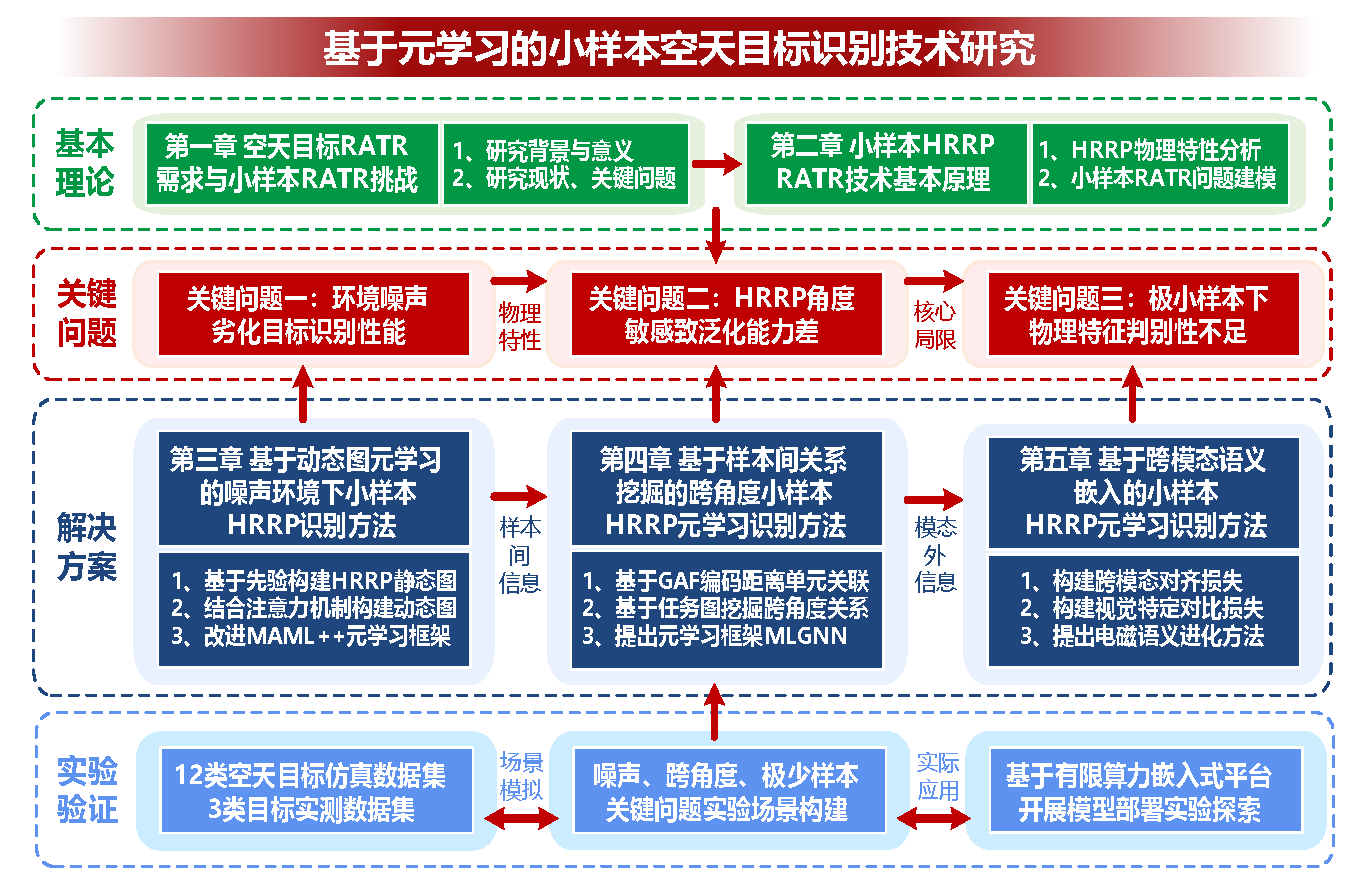
\includegraphics[width=\linewidth]{figures/general.pdf} % 假设图文件存在
    % \fbox{图 1.6: 本文组织架构和研究思路 (占位符)} % 使用占位符
    \caption{本文组织架构与研究思路框图}
    \label{fig:framework}
\end{figure}